\documentclass[]{book}
\usepackage{lmodern}
\usepackage{amssymb,amsmath}
\usepackage{ifxetex,ifluatex}
\usepackage{fixltx2e} % provides \textsubscript
\ifnum 0\ifxetex 1\fi\ifluatex 1\fi=0 % if pdftex
  \usepackage[T1]{fontenc}
  \usepackage[utf8]{inputenc}
\else % if luatex or xelatex
  \ifxetex
    \usepackage{mathspec}
  \else
    \usepackage{fontspec}
  \fi
  \defaultfontfeatures{Ligatures=TeX,Scale=MatchLowercase}
\fi
% use upquote if available, for straight quotes in verbatim environments
\IfFileExists{upquote.sty}{\usepackage{upquote}}{}
% use microtype if available
\IfFileExists{microtype.sty}{%
\usepackage{microtype}
\UseMicrotypeSet[protrusion]{basicmath} % disable protrusion for tt fonts
}{}
\usepackage[margin=1in]{geometry}
\usepackage{hyperref}
\hypersetup{unicode=true,
            pdftitle={The R in Spark},
            pdfauthor={Javier Luraschi},
            pdfborder={0 0 0},
            breaklinks=true}
\urlstyle{same}  % don't use monospace font for urls
\usepackage{natbib}
\bibliographystyle{apalike}
\usepackage{color}
\usepackage{fancyvrb}
\newcommand{\VerbBar}{|}
\newcommand{\VERB}{\Verb[commandchars=\\\{\}]}
\DefineVerbatimEnvironment{Highlighting}{Verbatim}{commandchars=\\\{\}}
% Add ',fontsize=\small' for more characters per line
\usepackage{framed}
\definecolor{shadecolor}{RGB}{248,248,248}
\newenvironment{Shaded}{\begin{snugshade}}{\end{snugshade}}
\newcommand{\KeywordTok}[1]{\textcolor[rgb]{0.13,0.29,0.53}{\textbf{#1}}}
\newcommand{\DataTypeTok}[1]{\textcolor[rgb]{0.13,0.29,0.53}{#1}}
\newcommand{\DecValTok}[1]{\textcolor[rgb]{0.00,0.00,0.81}{#1}}
\newcommand{\BaseNTok}[1]{\textcolor[rgb]{0.00,0.00,0.81}{#1}}
\newcommand{\FloatTok}[1]{\textcolor[rgb]{0.00,0.00,0.81}{#1}}
\newcommand{\ConstantTok}[1]{\textcolor[rgb]{0.00,0.00,0.00}{#1}}
\newcommand{\CharTok}[1]{\textcolor[rgb]{0.31,0.60,0.02}{#1}}
\newcommand{\SpecialCharTok}[1]{\textcolor[rgb]{0.00,0.00,0.00}{#1}}
\newcommand{\StringTok}[1]{\textcolor[rgb]{0.31,0.60,0.02}{#1}}
\newcommand{\VerbatimStringTok}[1]{\textcolor[rgb]{0.31,0.60,0.02}{#1}}
\newcommand{\SpecialStringTok}[1]{\textcolor[rgb]{0.31,0.60,0.02}{#1}}
\newcommand{\ImportTok}[1]{#1}
\newcommand{\CommentTok}[1]{\textcolor[rgb]{0.56,0.35,0.01}{\textit{#1}}}
\newcommand{\DocumentationTok}[1]{\textcolor[rgb]{0.56,0.35,0.01}{\textbf{\textit{#1}}}}
\newcommand{\AnnotationTok}[1]{\textcolor[rgb]{0.56,0.35,0.01}{\textbf{\textit{#1}}}}
\newcommand{\CommentVarTok}[1]{\textcolor[rgb]{0.56,0.35,0.01}{\textbf{\textit{#1}}}}
\newcommand{\OtherTok}[1]{\textcolor[rgb]{0.56,0.35,0.01}{#1}}
\newcommand{\FunctionTok}[1]{\textcolor[rgb]{0.00,0.00,0.00}{#1}}
\newcommand{\VariableTok}[1]{\textcolor[rgb]{0.00,0.00,0.00}{#1}}
\newcommand{\ControlFlowTok}[1]{\textcolor[rgb]{0.13,0.29,0.53}{\textbf{#1}}}
\newcommand{\OperatorTok}[1]{\textcolor[rgb]{0.81,0.36,0.00}{\textbf{#1}}}
\newcommand{\BuiltInTok}[1]{#1}
\newcommand{\ExtensionTok}[1]{#1}
\newcommand{\PreprocessorTok}[1]{\textcolor[rgb]{0.56,0.35,0.01}{\textit{#1}}}
\newcommand{\AttributeTok}[1]{\textcolor[rgb]{0.77,0.63,0.00}{#1}}
\newcommand{\RegionMarkerTok}[1]{#1}
\newcommand{\InformationTok}[1]{\textcolor[rgb]{0.56,0.35,0.01}{\textbf{\textit{#1}}}}
\newcommand{\WarningTok}[1]{\textcolor[rgb]{0.56,0.35,0.01}{\textbf{\textit{#1}}}}
\newcommand{\AlertTok}[1]{\textcolor[rgb]{0.94,0.16,0.16}{#1}}
\newcommand{\ErrorTok}[1]{\textcolor[rgb]{0.64,0.00,0.00}{\textbf{#1}}}
\newcommand{\NormalTok}[1]{#1}
\usepackage{longtable,booktabs}
\usepackage{graphicx,grffile}
\makeatletter
\def\maxwidth{\ifdim\Gin@nat@width>\linewidth\linewidth\else\Gin@nat@width\fi}
\def\maxheight{\ifdim\Gin@nat@height>\textheight\textheight\else\Gin@nat@height\fi}
\makeatother
% Scale images if necessary, so that they will not overflow the page
% margins by default, and it is still possible to overwrite the defaults
% using explicit options in \includegraphics[width, height, ...]{}
\setkeys{Gin}{width=\maxwidth,height=\maxheight,keepaspectratio}
\IfFileExists{parskip.sty}{%
\usepackage{parskip}
}{% else
\setlength{\parindent}{0pt}
\setlength{\parskip}{6pt plus 2pt minus 1pt}
}
\setlength{\emergencystretch}{3em}  % prevent overfull lines
\providecommand{\tightlist}{%
  \setlength{\itemsep}{0pt}\setlength{\parskip}{0pt}}
\setcounter{secnumdepth}{5}
% Redefines (sub)paragraphs to behave more like sections
\ifx\paragraph\undefined\else
\let\oldparagraph\paragraph
\renewcommand{\paragraph}[1]{\oldparagraph{#1}\mbox{}}
\fi
\ifx\subparagraph\undefined\else
\let\oldsubparagraph\subparagraph
\renewcommand{\subparagraph}[1]{\oldsubparagraph{#1}\mbox{}}
\fi

%%% Use protect on footnotes to avoid problems with footnotes in titles
\let\rmarkdownfootnote\footnote%
\def\footnote{\protect\rmarkdownfootnote}

%%% Change title format to be more compact
\usepackage{titling}

% Create subtitle command for use in maketitle
\newcommand{\subtitle}[1]{
  \posttitle{
    \begin{center}\large#1\end{center}
    }
}

\setlength{\droptitle}{-2em}
  \title{The R in Spark}
  \pretitle{\vspace{\droptitle}\centering\huge}
  \posttitle{\par}
  \author{Javier Luraschi}
  \preauthor{\centering\large\emph}
  \postauthor{\par}
  \predate{\centering\large\emph}
  \postdate{\par}
  \date{2018-02-21}

\usepackage{booktabs}
\usepackage{amsthm}
\makeatletter
\def\thm@space@setup{%
  \thm@preskip=8pt plus 2pt minus 4pt
  \thm@postskip=\thm@preskip
}
\makeatother

\usepackage{amsthm}
\newtheorem{theorem}{Theorem}[chapter]
\newtheorem{lemma}{Lemma}[chapter]
\theoremstyle{definition}
\newtheorem{definition}{Definition}[chapter]
\newtheorem{corollary}{Corollary}[chapter]
\newtheorem{proposition}{Proposition}[chapter]
\theoremstyle{definition}
\newtheorem{example}{Example}[chapter]
\theoremstyle{definition}
\newtheorem{exercise}{Exercise}[chapter]
\theoremstyle{remark}
\newtheorem*{remark}{Remark}
\newtheorem*{solution}{Solution}
\begin{document}
\maketitle

{
\setcounter{tocdepth}{1}
\tableofcontents
}
\chapter*{The R in Spark}\label{the-r-in-spark}
\addcontentsline{toc}{chapter}{The R in Spark}

In this book you will learn Apache Spark using R. The book intends to
take someone unfamiliar with Spark or R and help them become
intermediate users by teaching a set of tools, skills and practices
applicable to data science.

This work is licensed under the
\href{http://creativecommons.org/licenses/by-nc-nd/3.0/us/}{Creative
Commons Attribution-NonCommercial-NoDerivs 3.0} United States License.

\chapter{Introduction}\label{intro}

\href{https://en.wikipedia.org/wiki/Information_technology}{Humans have
been storing, retrieving, manipulating, and communicating information
since the Sumerians in Mesopotamia developed writing in about 3000 BC}.
Based on the storage and processing technologies employed, it is
possible to distinguish four distinct phases development: pre-mechanical
(3000 BC -- 1450 AD), mechanical (1450--1840), electromechanical
(1840--1940), and electronic (1940--present).

\href{https://en.wikipedia.org/wiki/Information_Age}{As humanity moves
from traditional industries to an economy based on information
technology} our footprint of digital information has kept growing at
\href{http://documents.worldbank.org/curated/en/896971468194972881/310436360_201602630200201/additional/102725-PUB-Replacement-PUBLIC.pdf}{exponential
rates}:

\includegraphics{bookdown-demo_files/figure-latex/unnamed-chunk-1-1.pdf}

With the ambition to provide a searchable tool to all this new digital
information, many companies attempted to provide such functionality with
what we now know as web search or search engines. Managing information
at this scale was a challenging problem that companies had to tackle
from the very beginning. Given the vast amount of digital information,
search engiens were unble to store all the web page information required
to support web searches in a single computer. This meant that they had
to split information across many machines, which was accomlished by
splitting this data and storing it as many files across many machines,
this approach became known as the Google File System from a research
paper published in 2003 by Google which has served for others to build
on.

One year later, in 2004, Google published a new paper describing how to
perform operations across the Google File System, this approach came to
be known as \textbf{MapReduce}. As you would expect, there are two
operations in MapReduce: Map and Reduce. We can think of the mapping
operation as a way to transform each file into a new file and, reuduce
as a way of combining two files into a new one. It happens to be the
case that using these two operations is sufficient to perform
interesting operations; for instance, MapReduce can be used to rank web
pages efficietly across a cluster of machines.

Since the papers were released by Google, a team in Yahoo worked on
implementing the Google File System and MapReduce as free open source
projects. This project was released in 2006 as \textbf{Hadoop} and the
Google File System became implemented as the Hadoop File System, or HDFS
for short. The Hadoop project made distributed file-based computing
accessible to many users and organizations.

While Hadoop provided support to perform map/reduce operations over a
distributed file system, it still required each map/reduce operation to
be written with code every time a data analysys was run. The
\textbf{Hive} project, released in 2008 by Facebook, brought Structured
Query Language (SQL) support to Hadoop. This meant that data analysis
could now be performed at large-scale without the need to write code for
each map/reduce operation, but instead, one could write generic data
analysis statements that are much easier to understand and write.

\section{Spark}\label{spark}

While Hadoop with Hive was a powerful tool, it was still working over a
distributed file system and was dependent on map/reduce operations. This
meant that it was running using disk drives which tend to be
significantly slower than using a computer's memory. In 2009, the
\textbf{Apache Spark} projects starts in Berkeley to improve over
Hadoop. Specifically, by making use of memory (instead of disk drives)
and by providing a richer set of verbs beyond map/reduce, this allowed
it to be much faster and generic than its predecessor. For instance, one
can
\href{https://databricks.com/blog/2014/11/05/spark-officially-sets-a-new-record-in-large-scale-sorting.html}{sort
100TB of data in 72min and 2100 computers using Hadoop, but only 206
computers in 23min using Spark}. Spark was build using the Scala
programming language, but interfaces to other programming languages are
also provided today. Spark was released as an open source project in
2010 with the scope of the project defined as follows:

\begin{quote}
``Apache Spark is a fast and general engine for large-scale data
processing.''

--- \href{http://spark.apache.org/}{spark.apache.org}
\end{quote}

meaning that Spark is a tool designed to support:

\begin{itemize}
\tightlist
\item
  \textbf{Data Processing}: Data processing is the collection and
  manipulation of items of data to produce meaningful information
  \citep{data-processing}.
\item
  \textbf{Large-Scale}: What \emph{large} means is hard to quantify, but
  one can interpret this as cluster-scale instead, which represents a
  set of connected computers that work together.
\item
  \textbf{General}: Spark optimizes and executes parallel generic code,
  as in, there is no restriction as to what type of code one can write
  in Spark.
\item
  \textbf{Fast}: Spark is much faster than it's predecesor by making
  efficient use of memory to speed data access while running algorithms
  at scale.
\end{itemize}

Spark is good at tackling large-scale data processing problems, this
usually known as \textbf{big data}
(\href{https://en.wikipedia.org/wiki/big_data}{data sets that are more
voluminous and complex that traditional ones}, but also is good at
tackling large-scale computation problems, known as \textbf{big compute}
(\href{https://www.nimbix.net/glossary/big-compute/}{tools and
approaches using a large amount of CPU and memory resources in a
coordinated way}). There is a third problem space where data nor compute
are necessarily large scale and yet, there are significant bennefits
from using the same tools.

Big data and big compute problems are usually easy to spot, if the data
does not fit into a single machine, you might have a big data problem;
if the data fits into a single machine but a process over the data takes
days, weeks or months to compute, you might have a big compute problem.

For the third problem space, there are a few use cases this breaks to:

\begin{enumerate}
\def\labelenumi{\arabic{enumi}.}
\item
  \textbf{Velocity}: One can have a dataset of 10GB in size and a
  process that takes 30min to run over this data, this is by no means
  big-compute nor big-data; however, if a data scientist is researching
  ways to improve accuracy for their models, reducing the runtime down
  to 3min it's a 10X improvement, this improvement can lead to
  significant advances and productivity gains by increasing the velocity
  at which one can analize data.
\item
  \textbf{Variery}: One can have an efficient process to collect data
  from many sources into a single location, usually a database, this
  process could be already running efficiently and close to realtime.
  Such processese are known at ETL (Extract-Transform-Load); data is
  extracted from multiple sources, transformed to the required format
  and loaded in a single data store. While this has worked for years,
  the tradeoff from this system is that adding a new data source is
  expensive, the system is centralized and tightly controlled. Since
  making changes to this type of systems could cause the entire process
  to come to a halt, adding new data sources usually takes long to be
  implemented. Instead, one can store all data its natural format and
  process it as needed using cluster computing, this architecture is
  currently known as a
  \href{https://en.wikipedia.org/wiki/Data_lake}{data lake}.
\end{enumerate}

Some people reffer to some of these bennefits as
\href{http://www.theserverside.com/feature/Handling-the-four-Vs-of-big-data-volume-velocity-variety-and-veracity}{the
four 'V's of big data}: Velocity, Variety, Volume and Veracity. Others
have gone as far as expending this to
\href{https://en.wikipedia.org/wiki/Big_data}{five} or even as
\href{https://tdwi.org/articles/2017/02/08/10-vs-of-big-data.aspx}{the
10 Vs of Big Data}. Mnemonics set aside, cluster computing is being used
today in more innovative ways and and is not uncommon to see
organizations experimenting with new workflows and a vareity of tasks
that were traditionally uncommon for cluster computing. Much of the hype
attributed to big data falls into this space, where some will argue that
everything should be considered big data and where others will argue
than almost nothing should. My hope is that this book will help you
understand the opportunities and limitations of Apache Spark with R.

\section{R}\label{r}

R is a computing language with it's inception dating back to Bell
Laboratories. At that time, computing was done by calling Fortran
subroutines which, apparently, were not pleasant to deal with. The S
computing language was designed as an interface language to support
higher abstractions to perform statistical computing over existing
subroutines:

\begin{figure}
\centering
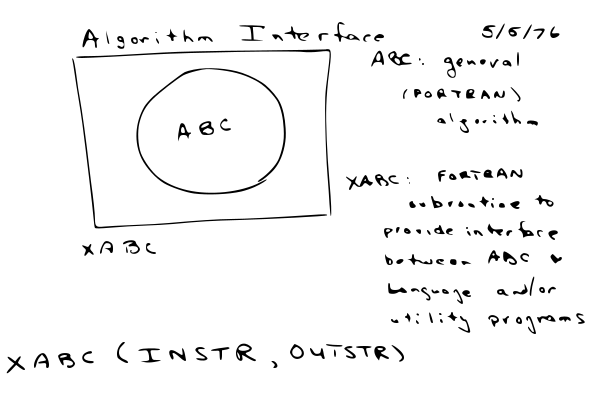
\includegraphics{images/01-intro-s-algorithm-interface.png}
\caption{Diagram by John Chambers - useR 2016}
\end{figure}

R is a modern and free implementation of S, specifically:

\begin{quote}
R is a programming language and free software environment for
statistical computing and graphics.

--- \href{https://www.r-project.org/}{The R Project for Statistical
Computing}
\end{quote}

There are two strong arguments for choosing R over other computing
languages while working with data:

\begin{itemize}
\tightlist
\item
  The \textbf{R Language} was designed by statisticians for
  statisticians, meaning, this is one of the few successful languages
  designed for non-programmers; so learning R will probably feel more
  natural. Additioanlly, since the R language was designed to be an
  interface to other tools and languages, R allows you to focus more on
  modeling and less on the pecularities of computer science and
  engineering.
\item
  The \textbf{R Community} provives a rich package archive provided by
  CRAN (\href{https://cran.r-project.org/}{The Comprehensive R Archive
  Network}) which allows you to install ready-to-use packages to perform
  many tasks, most notably, high-quality statistic models with many only
  available in R. In addition, the R community is a welcoming and active
  group of talented individuals motivited to help you succeed. Many
  packages provided by the R community make R, by far, the place to do
  statistical computing.
\end{itemize}

One can argue to what degree other fields, like machine learning,
overlap with statistics; so far, most people will argue that the overlap
is non-trivial. Similar arguments can be made for data science, big
data, deep learning and beyond. With the continuous rise of popularity
of R, I can only expect R's influence and scope to keep growing over
time; we can take a look at the historic downloads of R packages in CRAN
to get some sense of R's recent growth:

\includegraphics{bookdown-demo_files/figure-latex/unnamed-chunk-2-1.pdf}

\section{sparklyr}\label{sparklyr}

Back in 2016, there was a need in the R community to support Spark
through a clean interface compatible with other R packages and available
in CRAN. To this end, development of \texttt{sparklyr} started in 2016
by RStudio under JJ Allaire, Kevin Ushey and Javier Luraschi, version
0.4 was released in summer during the \emph{useR!} conference, this
first version added support for \texttt{dplyr}, \texttt{DBI}, modeling
with MLlib and an extenible API that enabled extensions like H2Os
\href{https://github.com/h2o/rsparkling}{rsparkling} package. Since
then, many new features have been added and support across many Spark
distributions and Cloud services hosting Apache Spark has made
available.

Officially,

\begin{quote}
\texttt{sparklyr} is an R interface for Apache Spark.

---\href{https://github.com/rstudio/sparklyr}{github.com/rstudio/sparklyr}
\end{quote}

It's available in CRAN and works like any other CRAN package, meaning
that: it's agnostic to versions, it's easy to install, it serves the R
community, it embraces other packages and practices from the R community
and so on. It's hosted in GitHub under
\href{github.com/rstudio/sparklyr}{https://github.com/rstudio/sparklyr}
and licensed under Apache 2.0 which is allows you to clone, modify and
contribute back to this project.

While thinking of who and why should use \texttt{sparklyr}, the
following roles come to mind:

\begin{itemize}
\tightlist
\item
  \textbf{New Users}: For new users, I'm going to argue that
  \texttt{sparklyr} is the best way to get started with Spark. My hope
  is that the first chapters of this book will get you up running with
  ease and set you up for long term success.
\item
  \textbf{Data Scientists}: I do believe, strongly, that
  \texttt{sparklyr} in combination with many other R packages and tools
  is the most productive environment for the modern data scientists.
  \texttt{sparklyr} allows support for high-level tasks and low-level
  extensibility mechanisms to match the needs and skills of every data
  scientists.
\item
  \textbf{Expert Users}: For those users that are already immersed in
  Spark and can write code natevely in Scala, I'm going to argue that
  making their work available as an \texttt{sparklyr} extension is very
  desirable for them and the community. The R community is one of the
  most welcoming and supportive communities I've known, so I can't think
  of better ways of helping the expert users share their work and
  knowledge than by making it available in CRAN to R community.
\end{itemize}

This book is titled ``The R in Spark'' as a way to describe and teach
that area of overlap between Spark and R. The R package that represents
this overlap is \texttt{sparklyr}; however, the overlap goes beyond a
package. It's an overlap of communities, expectations, future
directions, packages and package extensions as well. Naming this book
\texttt{sparklyr} or ``Introduction to sparklyr'' would have left behind
a much more exciting opportunity, an opportunity to present this book as
an intersection of the R and Spark communities. Both are solving very
similar problems with a set of different skills and backgrounds;
therefore, it is my hope that \texttt{sparklyr} can be a fertile ground
for innovation, a welcoming place to newcomers, a productive place for
experienced data scientists and an open community where cluster
computing and modeling can come together.

Here are some resources to help you get involved:

\begin{itemize}
\tightlist
\item
  \textbf{Documentation}: This should be your entry point to learn more
  about sparklyr, the documentation is kept up to date with examples,
  reference functions and many more relevant resources
  (\url{https://spark.rstudio.com}).
\item
  \textbf{Github}: If you believe something needs to get fixed, open a
  GitHub issue or send us a pull request
  (\url{https://github.com/rstudio/sparklyr}).
\item
  \textbf{Stack Overflow}: For general questions, Stack Overflow is a
  good place to start (\url{stackoverflow.com/tags/sparklyr}).
\item
  \textbf{Gitter}: For urgent issues or to keep in touch you can chat
  with us in Gitter (\url{https://gitter.im/rstudio/sparklyr}).
\end{itemize}

\chapter{Getting Started}\label{started}

For those already familiar with R, installing and launchiing Spark is as
easy as running:

\begin{Shaded}
\begin{Highlighting}[]
\KeywordTok{library}\NormalTok{(sparklyr)}

\KeywordTok{spark_install}\NormalTok{()}
\NormalTok{sc <-}\StringTok{ }\KeywordTok{spark_connect}\NormalTok{(}\DataTypeTok{master =} \StringTok{"local"}\NormalTok{)}
\end{Highlighting}
\end{Shaded}

For those new to R or to for those who want to gain deeper understanding
of the code above, this chapter will describe in detail how to get
started with R and Spark.

\section{Installation}\label{installation}

\subsection{Install R}\label{install-r}

\subsection{Install RStudio}\label{install-rstudio}

\subsection{Install Spark}\label{install-spark}

\section{Connection}\label{connection}

\section{Tools}\label{tools}

\chapter{Data Analysis}\label{dplyr}

\section{dplyr}\label{dplyr}

\section{DBI}\label{dbi}

\chapter{Modeling}\label{modeling}

\section{mllib}\label{mllib}

\chapter{Clusters}\label{clusters}

\section{On Prem}\label{on-prem}

\section{Cloud}\label{cloud}

\section{Livy}\label{livy}

\chapter{Data Sources}\label{data}

\section{CSV}\label{csv}

\section{Text}\label{text}

\section{Parquet}\label{parquet}

\section{JDBC}\label{jdbc}

\section{Others}\label{others}

\chapter{Extensions}\label{extensions}

\section{Using H2O}\label{using-h2o}

\section{Writting Extensions}\label{writting-extensions}

\chapter{Distributed R}\label{distributed}

\section{Use Cases}\label{use-cases}

\section{Troubleshooting}\label{troubleshooting}

\bibliography{book.bib,packages.bib}


\end{document}
